\section{Einleitung}
\setcounter{page}{1}
\pagenumbering{arabic}

\begin{figure}[h]
    \centering
    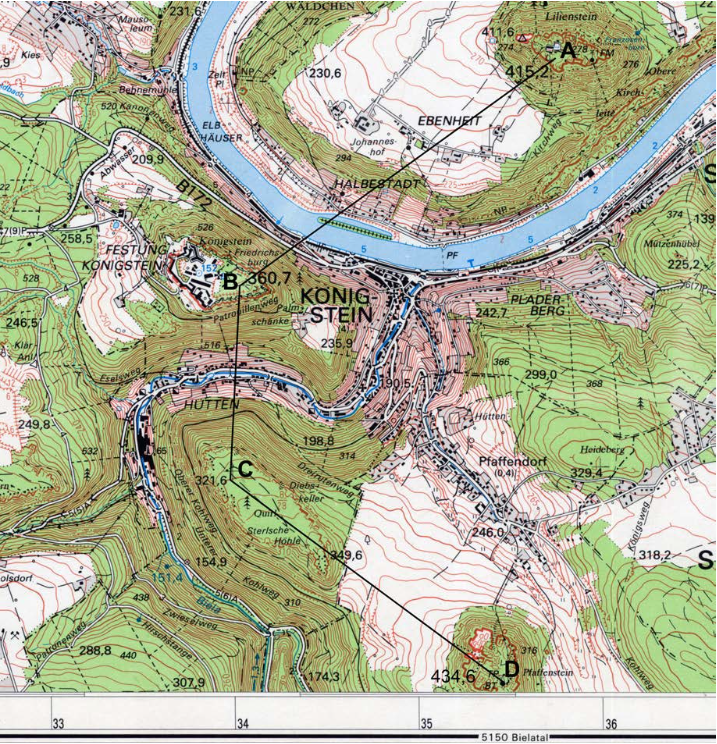
\includegraphics[scale = 0.5]{Abbildungen/5050_badschandau.png}
    \caption{Topographischen Karte Blatt 5050 „Bad Schandau“ \cite{landesvermessungsamt_sachsen_topographische_2009}}
    \label{fig:abb1}
\end{figure}

In der folgenden Abschlussaufgabe wird die Karte, aus Abbildung \ref{fig:abb1}, aus verschiedenen Blickwinkeln analysiert. Zuerst wird der Kartenmaßstab berechnet und durch Literatur bestätigt. Danach wird die in der Karte eingezeichnete Strecke von A (Lilienstein) über B (Königstein) und C(Quirl) bis D (Pfaffenstein) durch ein Höhenprofil ausgewertet.